% DNS defined in the intro!
\subsection{Incompressible DNS Application}
\label{sec:dns_full}

% Why DNS code needs to be improved
Direct numerical simulation (DNS) plays an important role in understanding turbulent flows because DNS provides highly fidelity data that is difficult in the experiments. After Kim et al. first used the DNS for wall-bounded turbulence flow in 1987 \cite{Kim:1987ub}, DNS has been used extensively to understand the turbulence phenomenon and to develop models of turbulence. DNS requires a large number of grids as Re increases. Therefore, the use of supercomputer is crucial to study the flow of high Re. To date, the highest $Re$ of the wall-bounded turbulence DNS is 250000, for which 242 billion degrees of freedom are used. \cite{Lee:2015er} However, Re = 5200 is also low compared to the high Re flow required for many engineering problems in our lives. For a DNS at higher Re, more advanced HPC system is required, and the DNS code should also be improved to the HPC system.


% Detail of simulation
In this section, we will show you the results of testing PoongBack on a KNL machine, which is a channel flow DNS code optimized for the modern supercomputers. PoongBack simulates the flow between two infinitely large parallel plates. Poongback consists of a 2D-decomposed parallel FFT and solving Navier-Stokes equation in the complex domain. More specifically, the 2D-decomposed parallel FFT consists of MPI communication for data alignment, data rearrangement before and after  MPI communication and each one-dimensional FFTs. On the other hand, in solving the N-S equation in the complex domain, it involves a large amount of linear equations and matrix-vector products. In order to solve the linear equations, Ax=b, we used a solver that was prepared separately without using the existing LAPACK library because A is a real band matrix and b and x are complex vectors.

Poongback, the DNS code for incompressible channel flow, has already shown excellent performance and has been already used in several researchers. Especially, it has been used for the simulation by \cite{Lee:2015er} and generating the data for virtual flow laboratory in Johns Hopkins Turbulence Data Base \cite{Graham:2015ha}. The spectral-Galerkin method and B-spline collocation method are used in PoongBack. There are four main parts in Poongback, data transpose with 2D decomposition, multiple 1D FFTs, solving linear equations with real matrix and complex vectors and I/O in HDF5 format. For I/O, we uses customized I/O library, ESIO \cite{Lee:2014ta}, but we have not tested its performance for this work. The data transpose 2D decomposition and multiple 1D FFTs are done by FFTW3.3 library. Note that FFTW3.3 (and above) library support the use of MPI but it is implemented for 1D data decomposition. To overcom this issue, we created two MPI-subcommunicators, and called FFTW for data transpose and FFTs seperately. Also, we have implemented customized banded-matrix solver to linear equations. See ref~\cite{Lee:2013kv} for more detail about PoongBack.

\begin{figure}[htb]
 \begin{center}
   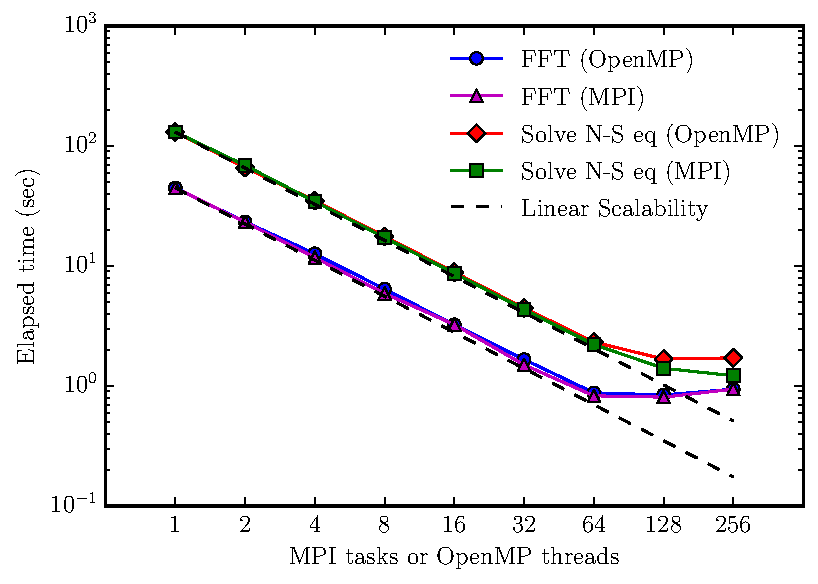
\includegraphics[width=0.45\textwidth]{DNS_FFT_Wave}
   \caption{Strong scaling result of 1D FFTs and Solving N-S equations in wavespeace for single timestep.}
   \label{fig:DNS_strong_scale_fft_wave}
 \end{center}
\end{figure}

% 1D FFT and wavespace performance

For this study the grid size is used $1024\times128\times512$ and the grid size is comparable for $Re_\tau = 180$ simulation by \cite{Kim:1987ub}. Throughout the every benchmark cases, the MCDRAM is used as a cache memory between processors and DRAM. Figure~\ref{fig:DNS_strong_scale_fft_wave} shows the strong scaling performance of 1D FFTs (real-to-complex, complex-to-real and complex-to-complex) and floating point operations with complex numbers including linear equation solvers. The linear equation, $A\mathbf{x} = \mathbf{b}$, is solved to compute B-spline coefficients. $A$ is a diagonal dominant banded matrix with additional non-zero elements in several top and bottom rows. $\mathbf{x}$ and $\mathbf{b}$ is complex vectors. As shown in the Figure~\ref{fig:DNS_strong_scale_fft_wave}, FFTs and floating point operations shows good scalability in both OpenMP only and MPI only cases with upto 64 processors. Using MPI only shows slightly better performance but the difference is negligible. After the hyperthread\todo{it this right term?} is used performance with FFTs are decreased because FFTs are bounded by the memory access not by floating point operations. On the otherhands, the kernel with linear equation shows slight performance increases even with the hyperthreads. Interestingly, using MPI shows better performance than OpenMP. This maybe due to the difference of memory access pattern between two parallelism. \todo{Chris, is this make sense?}.

% Transpose performance

\begin{figure}[htb]
 \begin{center}
   \includegraphics[width=0.45\textwidth]{DNS_Transpose}
   \caption{Strong scaling result of data reorder and MPI communication; OpenMP is not used.}
   \label{fig:DNS_strong_scale_transpose}
 \end{center}
\end{figure}

% Full timestep performance

\begin{figure}[htb]
 \begin{center}
   \includegraphics[width=0.45\textwidth]{DNS_Parallelism}
   \caption{Comparison of MPI$\times$OpenMP configuration}
   \label{fig:DNS_MPI_OpenMP}
 \end{center}
\end{figure}

\begin{figure}[htb]
 \begin{center}
   \includegraphics[width=0.45\textwidth]{DNS_full_timestep}
   \caption{Strong scaling result of total elapsed time for single timestep; (MPI tasks $\times$ OpenMP threads) is hybrid configuratation which showed  the best performance.}
   \label{fig:DNS_strong_scale_total_elapsed_time}
 \end{center}
\end{figure}





\todo{if we merge this with the previous section, we can have an intro
to dns and then talk about each in detail}

